\documentclass[
	a4paper,%
	11pt,% <10pt, 9pt>
	]{article}
	
\usepackage[english]{babel}
\usepackage{graphicx}
\usepackage{subcaption}
\usepackage{tabularx}
\usepackage{booktabs}
\usepackage{hyperref}
\urlstyle{same}


	
	
\begin{document}

\title{Agreement feature in Karrot - Writeup of process}

\author{Nathalie Szycher}
\date{\today}

\maketitle
\tableofcontents


\section{Introduction}

Karrot is a free and open-source software project run by community. The main idea is to help groups organise by starting a group on Karrot. Many Karrot groups are food sharing or saving groups, but the software is not limited to that. Whatever a groups vision or mission is, the Karrot projects supports communication, doing activities and group governance.

Within Karrot there is no admin structure as known from other software. Rights and in particular editing rights are handled by a trust system. This is one example how software interacts with group governance. But in most cases the groups are very independent to chose their own governance, agreements and rules. The challenge of the software is to support groups as best as possible.

The new agreements feature allows the group to save and store their agreements in one central place, accessible to every group member. This feature was subject of the first Karrot Community Design process, conducted from October 2020 to August 2021. The implementation described in this writeup is the latest iteration of the feature. This is part of the milestones for Karrot's funding from NGI0 Discovery Fund established by NLnet.



\section{Background}

This section covers the general meaning of governance and agreements for groups and in particular grass-root activists. It is shown how Karrot groups handle their agreements so far. Additionally the Google Sprint is introduced, which is the template for the Community Design Process within Karrot.

\subsection{Group Governance and Agreements}

Voluntary and activist groups often share the value of equity and aim for organising in a non-hierarchical and democratic way. To ensure this, especially when a group is growing or has the intention to grow, it is almost inevitable to write the processes a group is having (e.g. around decision making) down together with a shared statement around the vision and aims of a group. Typically this is covered in a governance agreement. Additionally, over time groups develop specific rules or policies around their activities. Every new member and also existing members should have access to these documents. They need to be transparent and public within a group, so every member can acknowledge them. In sociocracy, a way of decentralised decision making and organising, there is a concept called 'logbook'. It is the central place where an organisation can keep all their agreements, rules and policies. It is a great source of inspiration to review different agreements. A few Karrot groups made their governance document public in the community forum\footnote{\label{url:share_agreements2}\href{https://community.karrot.world/t/share-your-community-guidelines-rules-or-agreements}{https://community.karrot.world/t/share-your-community-guidelines-rules-or-agreements}}.
\subsection{Design Sprint}

The Design Sprint invented at Google is a process how a team can effectively work on a new project within five days typically from Monday to Friday\footnote{\label{url:google_sprint}\url{https://www.thesprintbook.com/}}\footnote{\label{url:google_sprint_gv}\url{https://www.gv.com/sprint/}}. All stages are shown in \autoref{fig:design-sprint}. The Design Sprint is well suited for software projects.

On the first day the challenge and the problem are defined. The team sets long-term goals for the project, but also looks at difficult questions for the sprint. A map of key players is drawn.  There is a set of methods the team can conduct like 'ask the experts' to gather more information in small interviews and 'how might we' to focus back on opportunities. At the end of the first day a target from the map is chosen.

The second day is all about getting ideas together and sketching solutions. At this point concrete drawings are welcome. As a guiding principle, every team member is asked to do their own sketching, inspired by existing solutions and the discussions from the previous days.

The different sketches will be presented to the team on the third day in order to decide for one or a mix of sketches. Later the day a storyboard will be produced to help prototyping. The storyboard shows in around ten steps how a user will interact with the new developed product.

The last two days are about prototyping. A prototype is build on the fourth day with enough functionality to allow user testing on the last day. On the last day interviews are done with users to see how the prototype lands with the people. The idea is to identify patterns from the interviews which can then be compare with the long-term goals and sprint questions from day one. On this basis the team can decide how to continue after the Design Sprint.

To have a successful Design Sprint among others there are two roles which needs to be assigned. One is the facilitator guiding the group through the whole process, knowing the steps and methods and bringing the team together. The second one is a decider, who is taking final decisions after the team went trough a non-binding voting phase.

\begin{figure}[ht]
	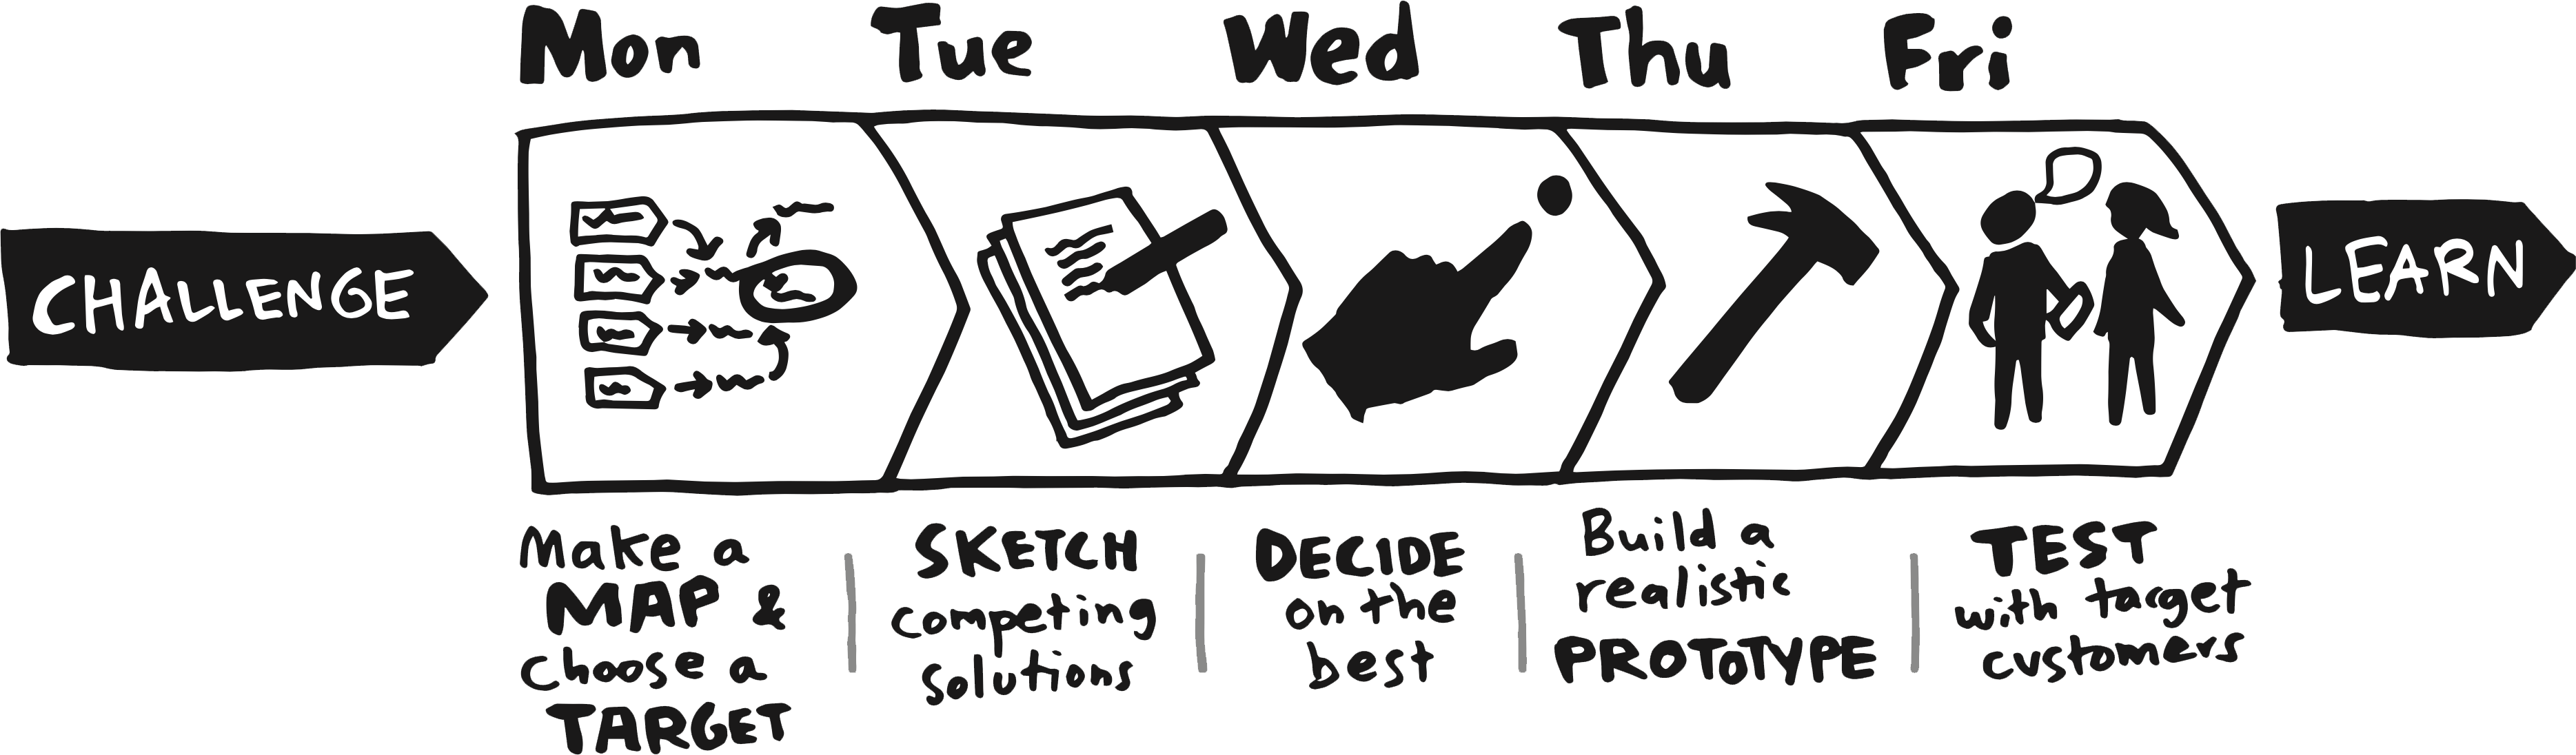
\includegraphics[width=\textwidth,
	]{images/sprint_process_overview.png}
	\caption[Overview of Design Sprint in five days]{Overview of Design Sprint in five days\footnote{\label{url:google_sprint_img}\url{https://www.thesprintbook.com/the-design-sprint/} on \today}.}
	\label{fig:design-sprint}
\end{figure}


\section{Community Design Process}

The agreement feature was designed using a Community Design Process. This is a variation of the Design Sprint adapted from the Karrot team and the Karrot Community. One of the most significant changes is to change the 'sprint' to a 'process'. The Community Design Process started in October 2020 and lasted until August 2021 with 5-6 team members and additional experts and Karrot users as interview partners. The following sections cover highlights and summaries taken from the Community forum. This writeup has a focus on outcomes, for a wider perspective on discussions and experiences the reader is encouraged to look into the meeting minutes and the various resources provided by the participants.


\subsection{Defining the Challenge}\label{subsec:challenge}

The first step of the design process is to define the challenge (see Stage 1 in the community forum\footnote{\label{url:1challenge}\url{https://community.karrot.world/t/stage-1-defining-the-challenge/534}}) in the context of a possible agreements feature and group governance in Karrot. As suggested by the Design Sprint a long-term goal is defined: “Karrot will facilitate groups in organizing and making decision in a democratic and transparent way, encouraging participation from all and avoiding the formation of unaccountable and fixed hierarchies between participants.”

Besides an optimistic long-term goal, more pessimistic process questions are asked:
\begin{itemize}
	\item How to encourage participation even from those less active in participating?
	\item How to encourage the people who are most active in participating and taking responsibility, while making them accountable for their actions and keeping them in check.
	\item How to be a complement for in-person meetings and other offline processes for making decisions, instead of something that would conflict and not combine well with these?
	\item How to enhance, rather than disturb, existing decision-making processes that groups already use?
\end{itemize}

After conducting several interviews with experts, in this case users of Karrot, five expressions are the distilled outcome following a 'how might we...' structure. These show the opportunities of the planned feature. 'How Might We...'
\begin{itemize}
	\item ...support groups to expand their governance model as they grow
	\item ...bring up delicate and important issues without exposing oneself (question of anonymity)
	\item ...make it easy for people to review existing rules
	\item ...bring new people into responsible roles
	\item ...make it easy for people to give more general feedback
\end{itemize}


\subsection{Sketching Solutions and Making a Decision}

The second stage is all about sketching ideas\footnote{\label{url:2sketching}\url{https://community.karrot.world/t/stage-2-sketching-solutions/589}}, first doing own sketches and then presenting them to the other participants. The defined long-term goal from \autoref{subsec:challenge} serves as a guideline and reference to come back to. This stage happened in several meetings and merged into a collaborative process to create a final sketch.

One idea coming up early on, is having a rule library. It is not only for a group to save their rules, but shared among Karrot groups to promote an exchange of ideas and experiences. Also the question how to add, review, change remove and discuss these rules is raised. Another idea is to make a feature where a group's vision and values are made explicit and to make it possible to connect rule making or collective agreements with those. Depending whether a group is well-established or newly arriving a Karrot, different guidance can be given around rules, agreements and vision. In \autoref{fig:sketch} a visualisation is shown, with different view of the feature. User can edit vision or rules and they are displayed in an agreements summary for the group, marked as published or pending. Published agreements could directly be shown in a inter-group space. Rules and agreements would go through a group process to progress from pending to published. This process can include a voting mechanism, a non-binding quick vote ('temperature check') or connect with the concept of trusted editors in Karrot, who then approve proposals. Overall four different screens need to be taken into consideration: list of agreements, agreement detail, agreement history and agreement proposal.
    

\begin{figure}[ht]
	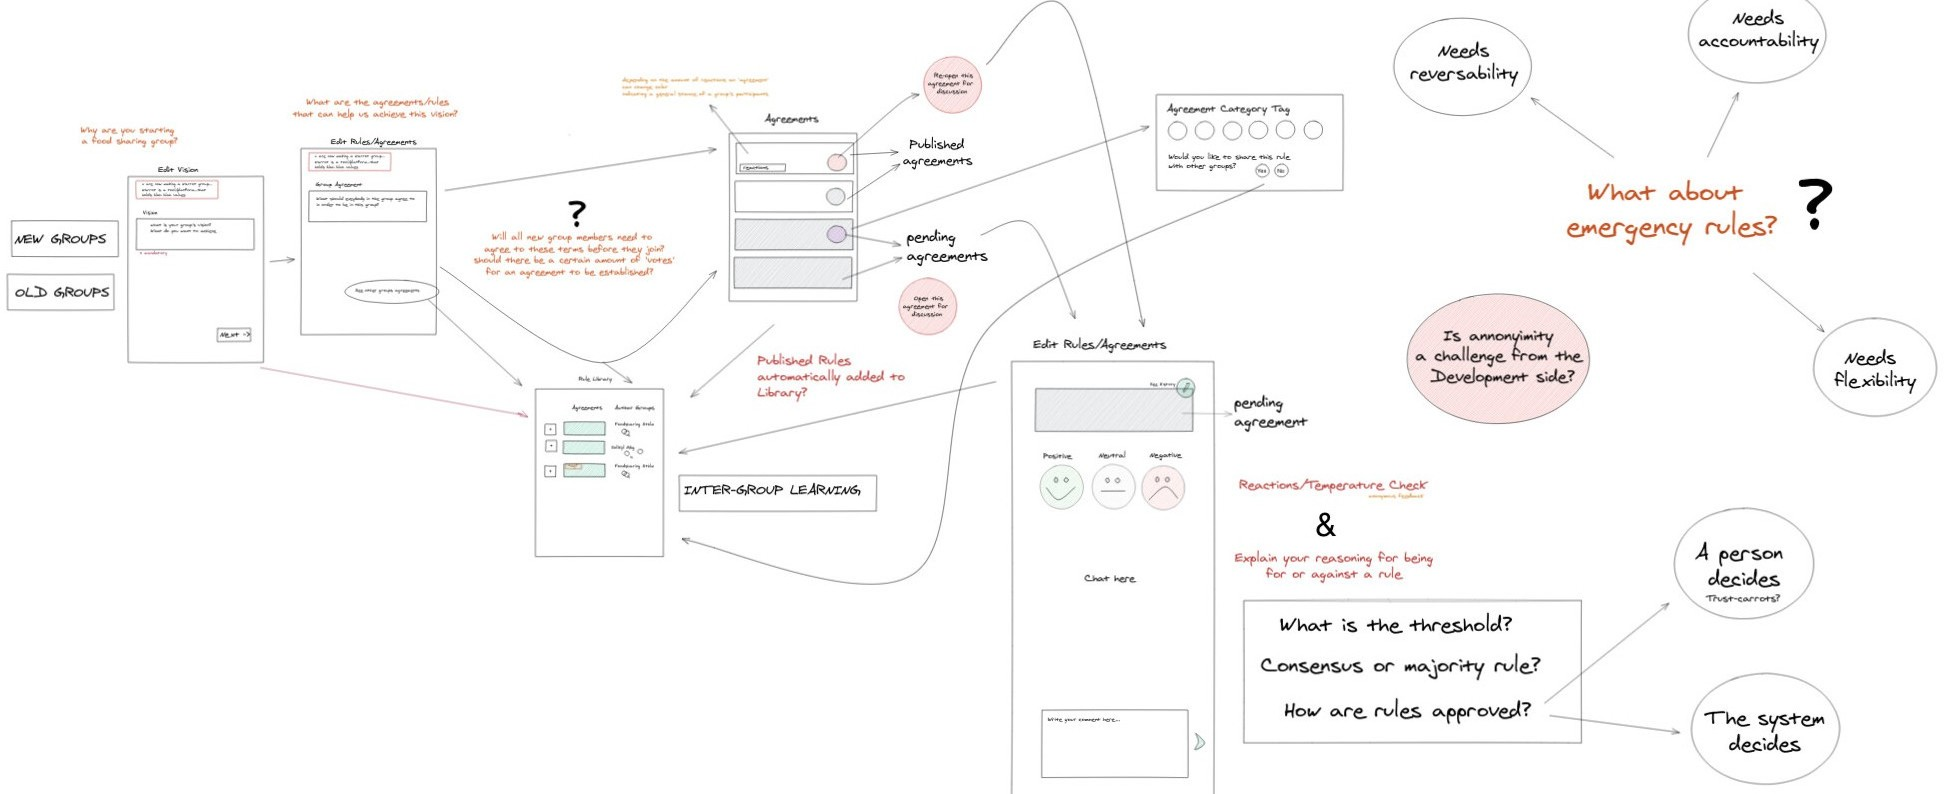
\includegraphics[width=\textwidth
	]{images/sketch.jpg}
	\caption{Sketching towards an agreements feature}
	\label{fig:sketch}
\end{figure}


Finishing the collaborative sketching phase, this is the decision\footnote{\label{url:3Decision}\url{https://community.karrot.world/t/stage-3-making-a-decision/608}} on which the prototype will be build:
\begin{itemize}
	\item only editors can submit proposals
	\item timescale: minimum 1 week + suggestions + custom → pick a specific date
	\item any editor can change the proposal. People get a notification of the change and are asked to review their vote
	\item everybody can vote
	\item score voting with negative weighting (2, 1, 0, -1, -2)
	\item anonymous voting
	\item negative votes require a reason and they’re kept anonymous (“explain why you don’t like it”)
	\item At least 5\% of members should vote for an agreement to get approved	
\end{itemize}

    
\subsection{Prototype}\label{subsec:prototype}

Based on the sketches and the decision a prototype was built: \url{https://karrot-prototyping.netlify.app} (see github repository\footnote{\label{url:prototype-github}\url{https://github.com/karrot-dev/karrot-prototyping}}). In the agreements view, there are two lists of agreements: approved and proposals. Approved proposals are marked with the date of approval and a detailed view can be opened. For proposals the voting phase is still open and the due date is indicated in the list. An example of a detailed view for a proposal is shown in \autoref{fig:screenshot-prototype}. Not only the proposal text is shown, but a chat for dicussion and also a voting option based on a score voting princile as used in a different KArrot fature\footnote{\label{url:score-vote}\href{https://community.karrot.world/t/info-how-does-the-conflict-resolution-feature-work/254/3}{https://community.karrot.world/t/info-how-does-the-conflict-resolution-feature-work/254/3}} with only one option available - the proposal. The negative voting option 'strong resistance' and 'resistance' counting -2 and -1 are only available if the user writes a message in the chat. After the discussion and voting phase, proposal which achive a total score above 0 are approved by the group.


For approved agreements a change can be proposed by the users. This will create a new proposal and a similar process is started as with a proposal from scratch. As an additional feature a diff view is provided, showing which lines or words have been added or removed. A completely new proposal is generated by clicking on the respective button and filling out the fields for time period, title, summary and text. After this step the new proposal is open for discussion and vote.

\begin{figure}[htb]
	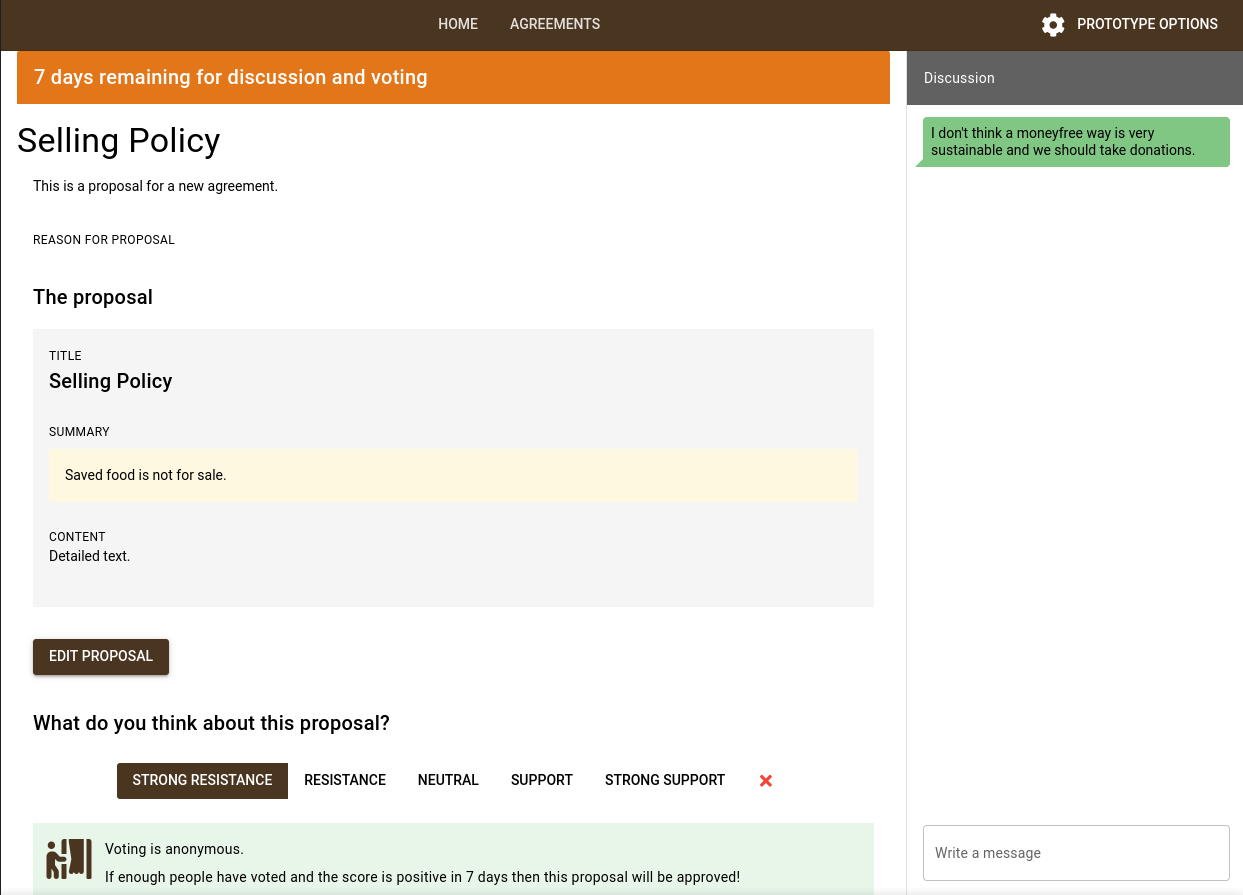
\includegraphics[width=\textwidth,
	]{images/screenshot-prototype.png}
	\caption{Screenshot of Prototype for Agreements feature, Proposal view}
	\label{fig:screenshot-prototype}
\end{figure}

\subsection{Testing the Prototype}

To get feedback from Karrot users in different group six interview where conducted with this testing protocol\footnote{\label{url:5Testing}\url{https://community.karrot.world/t/stage-5-testing-the-prototype/694}}:

\begin{itemize}
	\item Propose an existing document
		\begin{itemize}
			 \item Start with a written document that you want to use within your group
			 \item On the home page press “Start with empty data”
			 \item Make a proposal for the group to accept the document
		\end{itemize}
	\item Participate in an existing discussion
		\begin{itemize}
  			  \item Go back to the home page
  			  \item On the home page press “Start with sample data”
   			  \item Select an existing proposal
    			  \item Make a comment in the discussion
    		  	  \item Cast your vote
		\end{itemize}
	\item Change an existing agreement
		\begin{itemize}
   			 \item Select an existing agreement
    			 \item Read the agreement
    			 \item Propose a change
		\end{itemize}	
	
\end{itemize}

The latest version of the prototype described in \autoref{subsec:prototype} already is an iteration based on the given feedback. A few feature were removed or re-worked based on the user feedback. One example is the option to have value tags to the agreements such as 'fairness', 'respect', 'solidarity' or 'fun'. These were perceived as confusing and therefore removed. More feedback was given to the general appearance, to have more clarity between proposals and agreements. Another field of uncertainty lies in the editing of proposal: who gets to edit and what are the social norm around it. Users don't want to override or directly add to a existing proposal, a comment function or history of the change naming the author is preferred. In the prototype the voting page comes with a chat function, but to the groups it's an open question where the best place for discussion could be (in proposal, on group's wall, outside Karrot). A few comments where made around the voting system e.g. the negative voting and the question if it actually is revealing someone because user need to write in the chat first in order to give a negative vote. Overall this feature was perceived as useful, as it is a frequent question for a group how to come to a decision and where to store existing rules and agreements.


\subsection{Challenges and Reflection}

As one participant phrased it the whole process was rather a 'design thinking framework' than a sprint. The overall experience was positive, although a bit long. A steady team went through the step and had many meetings on the way, which contributed to a community vibe feeling. Especially in the beginning a shared understand of a very complex problem was reached and although not having answers to all the challenges and questions, it is good to have a general awareness around them. The length of the process and the time between meetings allowed more time to reflect. Also there was no pressure to be productive which contributed to the positive atmosphere. On the same point, it was difficult to keep the energy up throughout the whole time and the team is wondering how a follow-up can happen or what can bring a push to bring this feature forward and actually finish it. From an outside perspective the level of transparency and information provided in the community forum is remarkable and gives the reader a sense of the rich process. Aside from the time perspective, the way of decision making varies from the Google Sprint. In the Sprint there is an emphasis on efficiency and fast decision making, even bringing this into a designated role called 'Decider'. Whereas in Karrot the process ended up being very collaborative, with similar ideas merging together to outcomes for each step, where every participant could identify and agree with.



\section{Implementation}

The work on the agreements feature was resumed one year later which led to a first implementation in the software\footnote{\label{url:feature-github-front}\url{https://github.com/karrot-dev/karrot-frontend/pull/2593}}\footnote{\label{url:feature-github-back}\url{https://github.com/karrot-dev/karrot-backend/pull/1244}} . Many questions and blocking elements are connected to the voting and proposal part of the protoptype, whereas broad agreement exists that a list or library of agreements is useful to groups and their governance processes. Here is what the new feature adds (see \autoref{fig:screenshot-feature} to \ref{fig:screenshot-create-agreement})
\begin{itemize}
    \item editors can create and edit agreement
    \item everyone can view them
    \item list filtering by all or only active
    \item card or table view
    \item required fields: title, content, active from
    \item optional fields: summary, active to (putting this in the past makes it "inactive"), review date
    \item history view, in group history, plus at bottom of an agreement
    \item diff view for when particular fields change	
\end{itemize}

\begin{figure}[p]
\centering
\begin{subfigure}{0.3\textwidth}
\centering
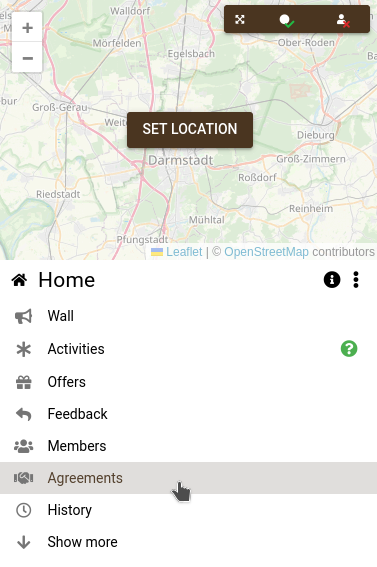
\includegraphics[width = \textwidth]{images/new-menu-item.png}
\caption{Main group menu}
\end{subfigure}
\begin{subfigure}{0.69\textwidth}
\centering
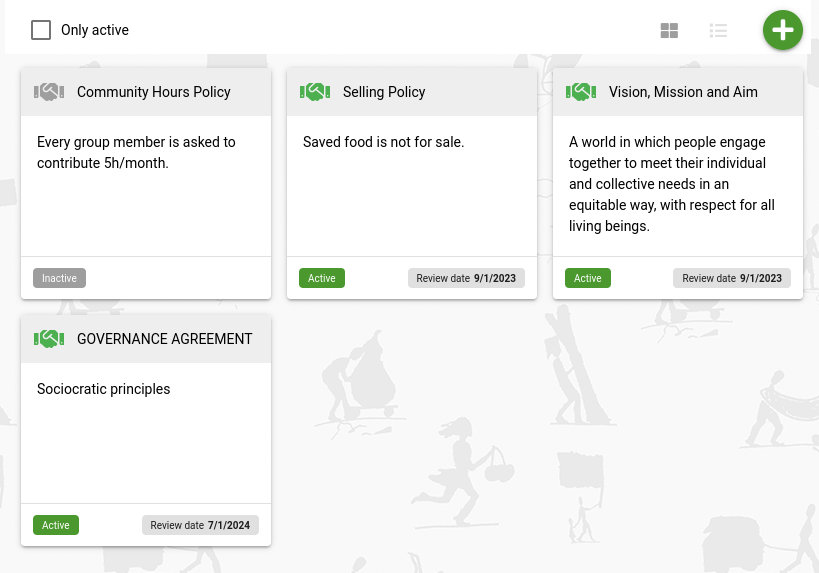
\includegraphics[width = \textwidth]{images/list-of-agreements.png}
\caption{List of group agreements}
\end{subfigure}
\caption{Screenshot of agreements feature implementation}
\label{fig:screenshot-feature}
\end{figure}


\begin{figure}[p]
	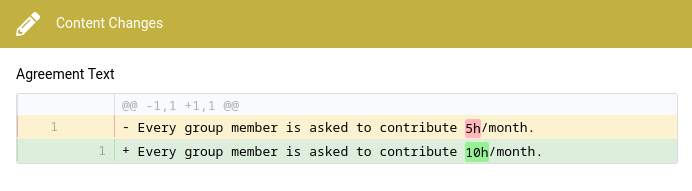
\includegraphics[width=.8\textwidth,
	]{images/changes-view.png}
	\caption{Screenshot of how changes of the proposal are shown in the history.}
	\label{fig:screenshot-changes}
\end{figure}

\begin{figure}[p]
\centering
	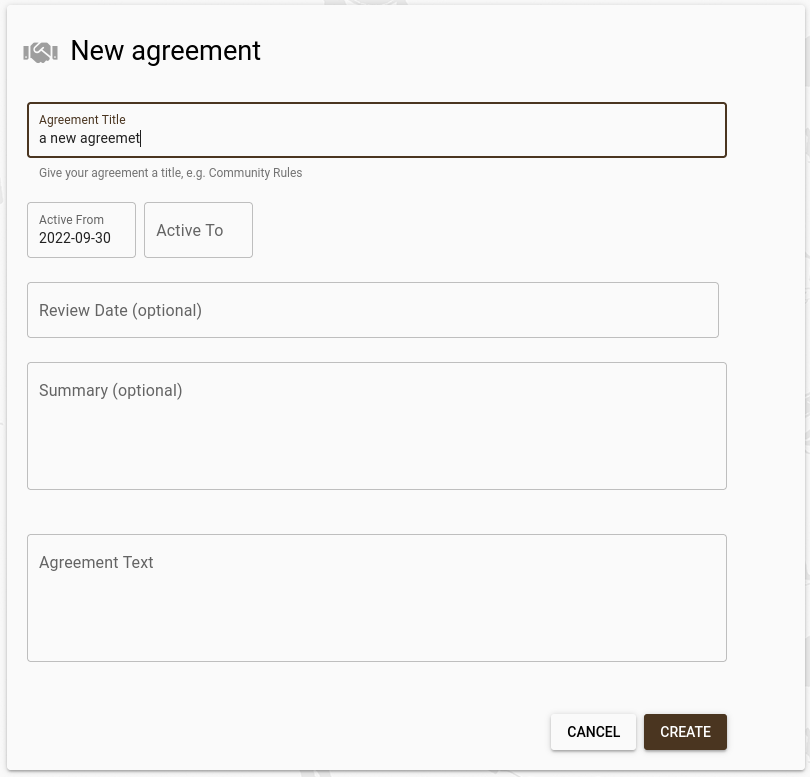
\includegraphics[width=0.6\textwidth,
	]{images/create_agreement.png}
	\caption{Screenshot of how to add new agreement}
	\label{fig:screenshot-create-agreement}
\end{figure}



\section{Conclusion and Outlook} \label{sec:outlook}

On the topic of agreements and group governance the first Karrot Community Design Process was conducted inspired by the Design Sprint. Within several meetings the challenge was defined, sketches were produced and merged and a prototype was developed and tested. Th final implementation led to an agreements list accessible from the group's main menu where every group agreement can be stored. Every editor of a Karrot group can add and edit agreement as part of their role.
Although the decision making is not represented on the software, as planned in the prototype, the new agreements feature brings the important question of group agreements into the focus of a group. Hopefully this will inspire groups to define their processes, make clear and transparent decisions and display them in a public place. Especially in large groups or groups with a decentralised power, it is important to have a well-maintained set of rules and agreements.
In the future the deciding part of an agreement can be put back into the focus, taking online and offline collaboration into account. It is a questions of balance and values of the Karrot project, how much and which types of decisions making and governance are promoted and embedded within the software. Additionally sharing and learning between different groups should be supported and enhanced e.g. what kind of agreements help a group to organise and grow. Theories like sociocracy and the experiences from the Karrot groups are worth to be explored further.


\end{document}
	
	
	